\documentclass[aspectratio=169]{beamer}
\setbeamertemplate{navigation symbols}{}
\setbeamertemplate{footline}[frame number]
\usefonttheme{professionalfonts}

\usepackage{amsmath,amssymb}
\usepackage{hyperref}
\usepackage{tikz}
\usepackage{pgfplots}
\pgfplotsset{compat=1.18}

\definecolor{segA}{RGB}{31,119,180}
\definecolor{segB}{RGB}{214,39,40}
\definecolor{envl}{RGB}{44,160,44}

\title{Unconstrained FPOP for Poisson Loss}
\subtitle{GSoC 2026 --- Medium Test}
\author{William Zhang}
\date{February 2026\\[6pt]
{\footnotesize\href{https://github.com/williamzhang7792/gsoc2026-gfpop-william-zhang/tree/main/2_medium}{github.com/williamzhang7792/gsoc2026-gfpop-william-zhang}}}

\begin{document}

\begin{frame}
\titlepage
\end{frame}

% ------------------------------------------------------------------
\begin{frame}{Optimal Partitioning}
Given count data $y_1,\dots,y_n$ and penalty $\beta > 0$, find the segmentation
minimizing
\[
  \sum_{k=1}^{K}\sum_{i\in S_k}\!\bigl(\mu_k - y_i\log\mu_k\bigr)
  \;+\; \beta\,(K-1)
\]
Each $\mu_k$ is set to the segment MLE $\bar{y}_{S_k}$.\\[2pt]
{\small(The constant $\log(y_i!)$ term is omitted---it does not depend on $\mu$ and cancels in optimization.)}

\pause\medskip

\textbf{Segment neighborhood} (\texttt{Segmentor3IsBack}):
best model for every $K = 1,\dots,K_{\max}$.\\[4pt]
\textbf{Optimal partitioning}: best model for a single $\beta$,
without computing all $K$.
\end{frame}

% ------------------------------------------------------------------
\begin{frame}{From $O(n^2)$ to $O(n)$: The FPOP Idea}
Standard DP: let $F_t ={}$ min penalized cost over $y_1,\dots,y_t$.
\[
  F_t = \min_{0\le\tau<t}\bigl\{F_\tau + C(y_{\tau+1:t}) + \beta\bigr\}
  \qquad\Longrightarrow\qquad O(n^2)
\]

\pause\medskip

\textbf{FPOP} (Maidstone et al.\ 2016):
keep cost as a \emph{function} of the segment mean.
\[
  Q_t(x) = \min\!\Big\{
    \underbrace{Q_{t-1}(x)}_{\text{continue}},\;
    \underbrace{\min_{x'}\!Q_{t-1}(x')+\beta}_{\text{switch}}
  \Big\}\;+\;\ell(y_t,x)
\]
where $x=\log\mu$ and $\ell(y,x) = e^x - yx$.

\pause\medskip

Notice that $Q_t$ is \textbf{piecewise} --- each piece inherits the
$ae^x + bx + c$ structure from the Poisson loss.
Candidates that fall entirely above the switch line get
pruned $\Rightarrow$ empirically $O(n)$.
\end{frame}

% ------------------------------------------------------------------
\begin{frame}{Three Operations Per Step}
\begin{enumerate}
\item \textcolor{segB}{\textbf{Flat line}} at
  $\displaystyle K_{t-1}+\beta$,\;
  where $K_{t-1}=\min_x Q_{t-1}(x)$
  \hfill{\small\texttt{set\_to\_unconstrained\_min\_of}}
\item \textcolor{envl}{\textbf{Min-envelope}} of continue curve
  and flat switch line
  \hfill{\small\texttt{set\_to\_min\_env\_of}}
\item \textbf{Add loss}\; $\ell(y_t, x) = e^x - y_t\, x$
\end{enumerate}

\pause\bigskip

Each $Q_t$ is stored as a linked list of pieces.\\[4pt]
Root-finding (Newton's method) determines where pieces cross.\\[4pt]
Backtracking recovers the optimal segmentation from $Q_n$.
\end{frame}

% ------------------------------------------------------------------
\begin{frame}{Constrained $\to$ Unconstrained}
\texttt{PeakSegOptimal}: 2 states (up/down), $N\times 2$ cost array.
\begin{itemize}
  \item \texttt{set\_to\_min\_less\_of}:
    enforces $\mu_k \le \mu_{k+1}$
  \item \texttt{set\_to\_min\_more\_of}:
    enforces $\mu_k \ge \mu_{k+1}$
\end{itemize}

\pause\medskip

My change: \textbf{one} state, $N\times 1$ cost array.
\begin{itemize}
  \item \texttt{set\_to\_unconstrained\_min\_of}:
    call \texttt{Minimize()}, emit a single constant piece
\end{itemize}

\pause\medskip

Everything else (min-envelope, root-finding, backtracking)
stays unchanged.
\end{frame}

% ------------------------------------------------------------------
\begin{frame}{Worked Example: The Data}
$\mathbf{y}=[3,\;3,\;10,\;10]$, \quad $\beta=2$.

\begin{center}
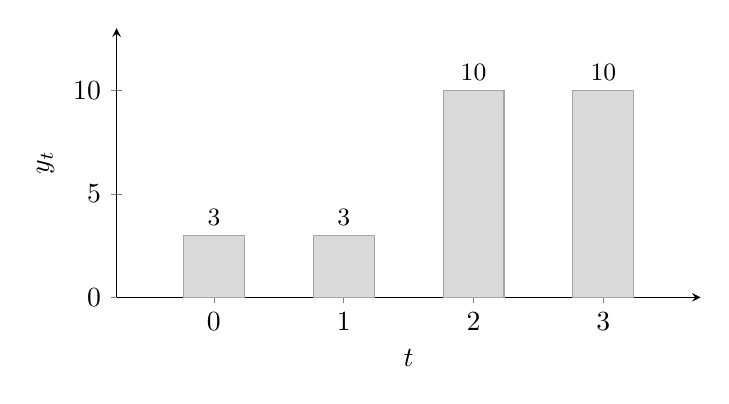
\begin{tikzpicture}
  \begin{axis}[
    ybar, bar width=22pt,
    width=9cm, height=5cm,
    ylabel={$y_t$},
    xlabel={$t$},
    xtick={0,1,2,3},
    ymin=0, ymax=13,
    nodes near coords,
    every node near coord/.append style={font=\small},
    axis lines=left,
    enlarge x limits=0.25,
  ]
  \addplot[fill=gray!30, draw=gray!70]
    coordinates {(0,3) (1,3) (2,10) (3,10)};
  \end{axis}
\end{tikzpicture}
\end{center}

Expected result: two segments $[3,3\mid 10,10]$
with means $\hat\mu_1=3$, $\hat\mu_2=10$.
\end{frame}

% ------------------------------------------------------------------
\begin{frame}{$t=0$: Initial Cost ($y_0=3$)}
\[
  Q_0(x) = e^x - 3x
\]

\begin{center}
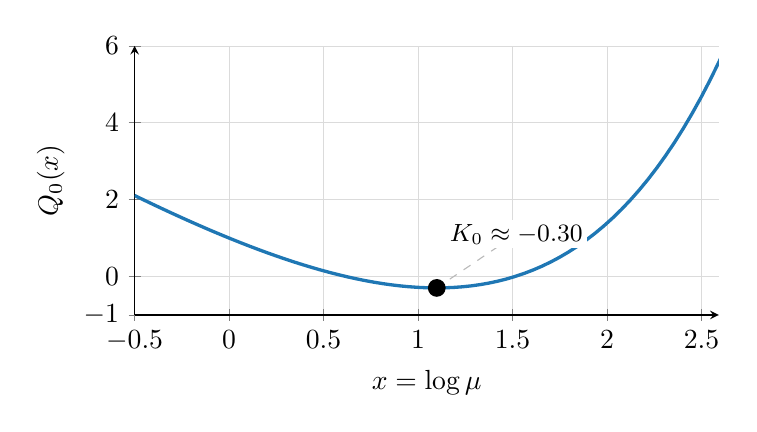
\begin{tikzpicture}
  \begin{axis}[
    width=9cm, height=5cm,
    domain=-0.5:3.2,
    samples=80,
    xlabel={$x=\log\mu$},
    ylabel={$Q_0(x)$},
    ymin=-1, ymax=6,
    ytick={-1,0,2,4,6},
    axis lines=left,
    grid=major,
    grid style={gray!28, very thin},
  ]
  \addplot[segA, very thick] {exp(x) - 3*x};
  \addplot[only marks, mark=*, mark size=3pt, black]
    coordinates {(1.099, -0.296)};
  \draw[gray!55, dashed, line width=0.4pt, shorten >=3pt, shorten <=2pt]
    (axis cs:1.52,1.1) -- (axis cs:1.099,-0.296);
  \node[font=\small, fill=white, inner sep=1.5pt] at (axis cs:1.52,1.1) {$K_0\approx -0.30$};
  \end{axis}
\end{tikzpicture}
\end{center}

Single piece.  Minimum $K_0\approx -0.30$ at $x=\log 3\approx 1.10$.
\end{frame}

% ------------------------------------------------------------------
\begin{frame}{$t=1$: Continue vs.\ Switch ($y_1=3$)}
\begin{columns}[T]
\begin{column}{0.57\textwidth}
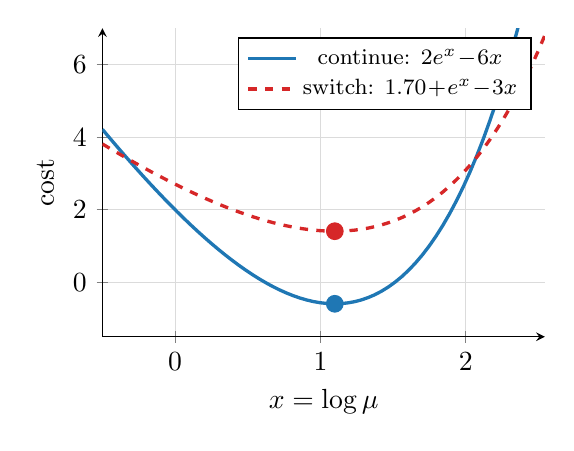
\begin{tikzpicture}
  \begin{axis}[
    width=7.2cm, height=5.5cm,
    domain=-0.5:3.2,
    samples=80,
    xlabel={$x=\log\mu$},
    ylabel={cost},
    ymin=-1.5, ymax=7,
    axis lines=left,
    grid=major,
    grid style={gray!28, very thin},
    legend pos=north east,
    legend style={font=\footnotesize},
  ]
  \addplot[segA, very thick] {2*exp(x) - 6*x};
  \addlegendentry{continue: $2e^x\!-\!6x$}
  \addplot[segB, very thick, dashed] {1.704 + exp(x) - 3*x};
  \addlegendentry{switch: $1.70\!+\!e^x\!-\!3x$}
  \addplot[only marks, mark=*, mark size=3pt, segA]
    coordinates {(1.099, -0.592)};
  \addplot[only marks, mark=*, mark size=3pt, segB]
    coordinates {(1.099, 1.408)};
  \end{axis}
\end{tikzpicture}
\end{column}
\begin{column}{0.41\textwidth}
\textbf{Continue} $[3,3]$:\\
$\min\approx -0.59$ at $\mu=3$

\medskip

\textbf{Switch} (new seg $[3]$):\\
$\min\approx 1.41$ at $\mu=3$

\medskip

Continue wins by $\approx 2$.

\medskip

\textit{Data is consistent---no reason to split.}

\medskip

$K_1 \approx -0.59$
\end{column}
\end{columns}
\end{frame}

% ------------------------------------------------------------------
\begin{frame}{$t=2$: The Jump ($y_2=10$)}
\begin{columns}[T]
\begin{column}{0.57\textwidth}
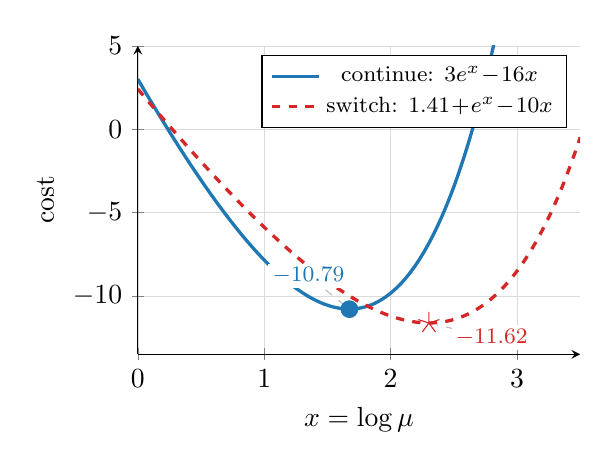
\begin{tikzpicture}
  \begin{axis}[
    width=7.2cm, height=5.5cm,
    domain=0:3.5,
    samples=100,
    xlabel={$x=\log\mu$},
    ylabel={cost},
    ymin=-13.5, ymax=5,
    axis lines=left,
    grid=major,
    grid style={gray!28, very thin},
    legend pos=north east,
    legend style={font=\footnotesize},
    clip=true,
  ]
  \addplot[segA, very thick] {3*exp(x) - 16*x};
  \addlegendentry{continue: $3e^x\!-\!16x$}
  \addplot[segB, very thick, dashed] {1.408 + exp(x) - 10*x};
  \addlegendentry{switch: $1.41\!+\!e^x\!-\!10x$}
  \addplot[only marks, mark=*, mark size=3pt, segA]
    coordinates {(1.674, -10.79)};
  \addplot[only marks, mark=star, mark size=4pt, segB]
    coordinates {(2.303, -11.62)};
  \draw[gray!55, dashed, line width=0.4pt, shorten >=3pt, shorten <=2pt]
    (axis cs:1.35,-8.8) -- (axis cs:1.674,-10.79);
  \node[segA, font=\footnotesize, fill=white, inner sep=1.5pt]
    at (axis cs:1.35,-8.8) {$-10.79$};
  \draw[gray!55, dashed, line width=0.4pt, shorten >=3pt, shorten <=2pt]
    (axis cs:2.8,-12.5) -- (axis cs:2.303,-11.62);
  \node[segB, font=\footnotesize, fill=white, inner sep=1.5pt]
    at (axis cs:2.8,-12.5) {$-11.62$};
  \end{axis}
\end{tikzpicture}
\end{column}
\begin{column}{0.41\textwidth}
\textbf{Continue} $[3,3,10]$:\\
$\min\approx -10.79$ at $\mu\approx 5.3$

\medskip

\textbf{Switch} $[3,3\mid 10]$:\\
$\min\approx -11.62$ at $\mu=10$ \;$\star$

\medskip

\textbf{Switch wins.}

\medskip

$y_2=10$ deviates far from $\bar{y}_{0:1}=3$:
paying $\beta=2$ to start fresh is worth it.

\medskip

Curves cross at $x\approx 1.82$.
\end{column}
\end{columns}
\end{frame}

% ------------------------------------------------------------------
\begin{frame}{Result}
\begin{columns}[T]
\begin{column}{0.55\textwidth}
\begin{center}
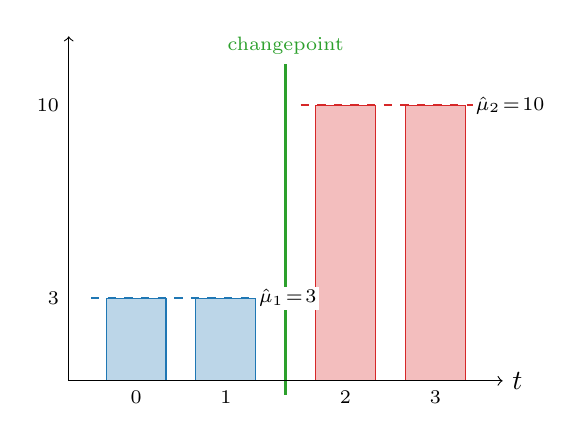
\begin{tikzpicture}[xscale=0.95, yscale=0.35]
  % segment 1
  \fill[segA!30, draw=segA] (0,0) rectangle (0.8,3);
  \fill[segA!30, draw=segA] (1.2,0) rectangle (2.0,3);
  % segment 2
  \fill[segB!30, draw=segB] (2.8,0) rectangle (3.6,10);
  \fill[segB!30, draw=segB] (4.0,0) rectangle (4.8,10);
  % means
  \draw[segA, thick, dashed] (-0.2,3) -- (2.0,3);
  \draw[segB, thick, dashed] (2.6,10) -- (4.9,10);
  % changepoint
  \draw[envl, very thick] (2.4,-0.5) -- (2.4,11.5);
  \node[envl, above, font=\scriptsize] at (2.4,11.5) {changepoint};
  % mean labels on top so not covered; white fill for clarity
  \node[font=\scriptsize, fill=white, inner sep=1pt] at (2.0,3) [right] {$\hat\mu_1\!=\!3$};
  \node[font=\scriptsize, fill=white, inner sep=1pt] at (4.9,10) [right] {$\hat\mu_2\!=\!10$};
  % axes
  \draw[->] (-0.5,0) -- (5.3,0) node[right] {$t$};
  \draw[->] (-0.5,0) -- (-0.5,12.5);
  \foreach \i/\x in {0/0.4, 1/1.6, 2/3.2, 3/4.4}
    \node[below, font=\scriptsize] at (\x,0) {$\i$};
  \foreach \y in {3,10}
    \node[left, font=\scriptsize] at (-0.5,\y) {\y};
\end{tikzpicture}
\end{center}
\end{column}
\begin{column}{0.43\textwidth}
\textbf{Backtracking:}
\begin{enumerate}
  \item $t\!=\!3$: best mean $\mu\!=\!10$,\\
        prev seg end $= 1$
  \item $t\!=\!1$: best mean $\mu\!=\!3$,\\
        prev seg end $= -1$ (start)
\end{enumerate}

\medskip

Two segments:\\[2pt]
$S_1 = \{y_0, y_1\}$, $\hat\mu_1 = 3$\\
$S_2 = \{y_2, y_3\}$, $\hat\mu_2 = 10$

\medskip

Penalized cost $\approx -24.64$.
\end{column}
\end{columns}
\end{frame}

% ------------------------------------------------------------------
\begin{frame}{Why Pruning is Exact}
At step $t$, candidate $\tau$ is pruned if
\[
  Q_t(x,\tau) \;\ge\; K_t + \beta
  \quad\text{for all } x
\]
i.e., continuing from $\tau$ is worse than starting fresh,
for \emph{every} possible mean.

\pause\bigskip

\textbf{Claim}: a pruned candidate can never become optimal again.

\pause\medskip

\begin{enumerate}
\item At time $t$: candidate $\tau$ is replaced by $\tau'\!=\!t$,
  so $Q_t(x,\tau) > Q_t(x,\tau')$ for all $x$.
\item Future data adds the same loss to both:
\[
  Q_{t+s}(x,\tau) = Q_t(x,\tau) + L(x)
  \;>\; Q_t(x,\tau') + L(x) = Q_{t+s}(x,\tau')
\]
\item Even if a future $K_{t+s}$ is huge,
  $\tau$ still loses to $\tau'$ (which is alive).
\end{enumerate}

\pause\medskip

$\Rightarrow$ Pruned = dead forever.  FPOP is \textbf{exact}.
\end{frame}

% ------------------------------------------------------------------
\begin{frame}{Pruning in Practice: Why $O(n)$}
Consider a flat signal ($y_t = c$ for all $t$):

\begin{itemize}
  \item The original candidate $\tau\!=\!0$ is the global optimum
    $\to$ never pruned.
  \item Each new ``switch'' candidate $\tau\!=\!t$ pays penalty $\beta$
    but gains no advantage on flat data.
  \item As flat data accumulates, the false start's cost rises
    above $K+\beta$.
  \item It gets pruned $\to$ active candidate list stays small
    (often 2--3 pieces).
\end{itemize}

\pause\bigskip

In general: the list grows when the signal changes,
and shrinks (via pruning) when it stabilizes.\\[4pt]
Amortized over the whole sequence: empirically $O(n)$.
\end{frame}

% ------------------------------------------------------------------
\begin{frame}{Seeing a Pruning Step}
\begin{columns}[T]
\begin{column}{0.44\textwidth}
At each step the active set holds one cost curve per
surviving candidate.

\medskip

The flat line at $K_t+\beta$ is the \textbf{ceiling}:
if a candidate's curve sits entirely above it,
that candidate is dead---it can never win for any
future~$\mu$.

\medskip

\textcolor{segA}{Candidate $\tau_1$} dips below
$\to$ survives.\\[2pt]
\textcolor{gray}{Candidate $\tau_2$} is entirely above
$\to$ \textbf{pruned}.

\medskip

On flat signals, new candidates are quickly pruned
$\to$ the active set stays small $\to$ empirical $O(n)$.
\end{column}
\begin{column}{0.54\textwidth}
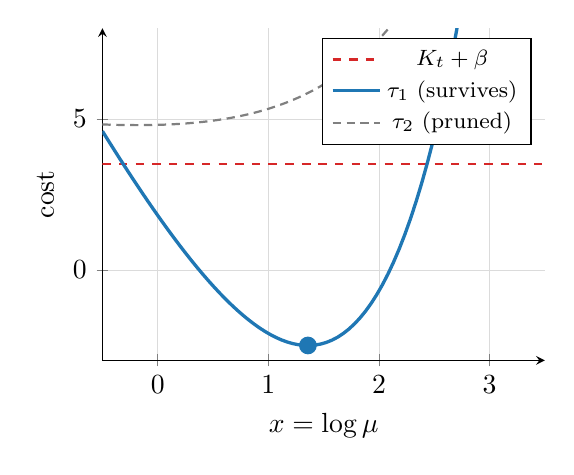
\begin{tikzpicture}
  \begin{axis}[
    width=7.2cm, height=5.8cm,
    domain=-0.5:3.5,
    samples=80,
    xlabel={$x=\log\mu$},
    ylabel={cost},
    ymin=-3, ymax=8,
    axis lines=left,
    grid=major,
    grid style={gray!28, very thin},
    legend pos=north east,
    legend style={font=\footnotesize},
    clip=true,
  ]
  % switch ceiling
  \addplot[segB, thick, dashed] {3.5};
  \addlegendentry{$K_t+\beta$}
  % candidate tau_1: dips below the line
  \addplot[segA, very thick] {1.8*exp(x) - 7*x};
  \addlegendentry{$\tau_1$ (survives)}
  % candidate tau_2: entirely above
  \addplot[gray, thick, densely dashed] {0.6*exp(x) - 0.5*x + 4.2};
  \addlegendentry{$\tau_2$ (pruned)}
  % mark the survivor's minimum
  \addplot[only marks, mark=*, mark size=3pt, segA]
    coordinates {({ln(7/1.8)}, {1.8*(7/1.8) - 7*ln(7/1.8)})};
  % "pruned" annotation on tau_2
  \node[gray, font=\footnotesize, fill=white, inner sep=1.5pt]
    at (axis cs:2.5,5.8) {pruned};
  \draw[gray, dashed, line width=0.4pt, shorten >=3pt, shorten <=2pt]
    (axis cs:2.5,5.8) -- (axis cs:2.2,5.0);
  \end{axis}
\end{tikzpicture}
\end{column}
\end{columns}
\end{frame}

% ------------------------------------------------------------------
\begin{frame}{Implementation}
Starting from \texttt{PeakSegOptimal}:

\begin{itemize}
  \item \textbf{Reused}: \texttt{PoissonLossPieceLog},
    \texttt{PiecewisePoissonLossLog},
    \texttt{set\_to\_min\_env\_of}, \texttt{Minimize},
    root-finding, \texttt{findMean}
  \item \textbf{New}: \texttt{set\_to\_unconstrained\_min\_of}
    (7 lines---just \texttt{Minimize} + emit flat piece)
  \item \textbf{Simplified}: 2-state DP loop $\to$ 1-state,
    $N\!\times\!2 \to N\!\times\!1$
  \item \textbf{Added}: Rcpp wrapper, input validation, backtracking
\end{itemize}

\pause\bigskip

Self-contained: \texttt{PoissonFPOP.cpp} ($\sim$760 lines,
mostly reused infrastructure).\\[4pt]
\texttt{sourceCpp("PoissonFPOP.cpp")} --- no package install needed.
\end{frame}

% ------------------------------------------------------------------
\begin{frame}{Validation}
Compared against
\texttt{Segmentor3IsBack::Segmentor(model=1)}
using \texttt{testthat}.\\[4pt]
8 test cases, 54 assertions:

\medskip

\begin{tabular}{ll}
3-segment data & penalties 5, 10, 50, 100 \\
Single changepoint & penalties 10, 50, 200 \\
Constant-rate data & penalty 500 (1 segment) \\
5-segment data & penalties 1, 5, 20, 100 \\
Data with zeros & penalties 1, 5, 50 \\
$\beta=0$ & every point its own segment \\
$n=2$ & 1-segment and 2-segment outcomes \\
Bad input & negative data, all-identical data \\
\end{tabular}

\bigskip

\textbf{All breakpoints and segment means match exactly.}\\[6pt]
Same results as Segmentor's $O(K_{\max}\, n^2)$ segment neighborhood,
but in empirical $O(n)$.
\end{frame}

\end{document}
